We have thus far described the likelihood,
$\Prob(X | N, \ell, f)$, and specified the prior, $\Prob(N, \ell, f)$. 
For moment, we treat the model parameters, the background and PSF, as known and fixed
(we can use the SDSS estimates, for example). In section~\ref{sec:model_params}, we extend to unknown 
model parameters and estimate them as part of our inference procedure. 

We seek the posterior distribution 
$\Prob(N, \ell, f | X)$. In most nontrivial probabilistic models, including ours, the exact posterior distribution is intractable.

Markov chain Monte Carlo (MCMC) is a common approach for approximating
posterior distributions by constructing a stochastic process on the parameter space whose stationary distribution is the true posterior. 
However, its computational cost is prohibitively expensive for
large-scale astronomical surveys. Instead, we propose to construct an approximate posterior using variational inference, resulting in a procedure that is several orders of magnitude faster than MCMC.

Variational inference~\cite{Blei_2017_vi_review, Jordan_intro_vi, Wainwrite_graph_models_vi}
posits a family of distributions $\mathcal{Q}$ and seeks
the distribution $q^*\in \mathcal{Q}$ that is closest to the true posterior
in $\KL$ divergence. Suppose the family of distributions $\mathcal{Q}$ is parameterized by a real-valued vector $\eta$. The objective is 
\begin{align}
   \eta^* &= \argmin_{\eta} \Big\{ \mathrm{KL}\Big[\,q_\eta(N, \ell, f | X)\, \| \,\Prob(N, \ell, f | X )\,\Big]\Big\} 
   \label{eq:kl_objective}
\end{align}

We note that minimizing the $\KL$ divergence is equivalent to maximizing the ELBO (evidence lower bound), defined as 
\begin{align}
    \mathcal{L} = 
    \Expect_{q_\eta(N, \ell, f | X)}\Big[\log\Prob(X, N, \ell, f) - \log q_\eta(N, \ell, f | X)\Big],
    \label{eq:elbo}
\end{align}
which does not depend on the marginal data distribution $\Prob(X)$, which is intractable. 

\subsection{The variational distribution}
We now describe our family of distributions $\mathcal{Q}$. 
In the traditional variational inference setup, 
$q_\eta$ depends on data $X$ only through the optimization objective 
(so $q_\eta(N, \ell, f | X)$,
becomes $q_\eta(N, \ell, f)$ with no dependence on $X$). 
Here, we take an amortized approach where
$q_\eta$ explicitly depends on data $X$. Specifically, a neural network 
maps input data $X$ to distributional parameters of $(N, \ell, f)$ 
under $q$. The variational parameters $\eta$ in equation~\eqref{eq:kl_objective} 
are the neural network weights. 
In the ensuing subsections, we detail the construction of our variational distribution. 

\subsubsection{The factorization}
To make the objective in equation~\eqref{eq:kl_objective} tractable in most 
applications, the family $\mathcal{Q}$ is restricted to probability distributions 
that limit conditional dependencies between latent variables. In the most extreme case, mean-field variational inference, 
the distribution over latent variables is assumed to fully factorize in the approximate posterior. 

Our factorization takes a spatial structure: we first decompose the full 
$H \times W$ image into disjoint $s \times s$ tiles. 
Independently for each tile,
we infer the number, locations, and fluxes of stars falling in that tile.
Let $k = 1, ..., K$ index the tiles. Then
denote the number of stars on tile $k$ by $N^k$;
the locations by $\ell^k = (\ell_{N, i}^k)_{i \leq N}$; 
the fluxes $f^k = (f_{N, i}^k)_{i \leq N}$. Recall that locations on the 
full image $\ell_{N, i}$ are parameterized to be in $[0, H] \times [0, W]$; 
locations on the tiles $\ell^k_{N, i}$ parameterized to be in
$[0, s] \times [0, s]$. A schematic 
of our tiling is shown in figure~\ref{fig:ex_tiles}. 

\begin{figure}[h]
    \centering
    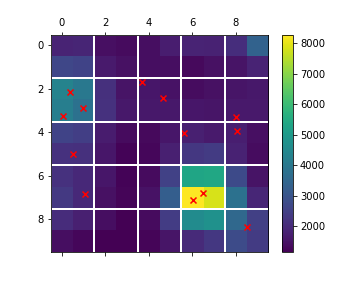
\includegraphics[width = 0.5\textwidth]{figures/example_tiled.png}
    \vspace{-1cm}
    \caption{Tiling a 10 x 10 image into 2 x 2 patches. }
    \label{fig:ex_tiles}
\end{figure}

Note that there is a bijection between latent variables on each tile and latent variables on the full image (locations on the full image map to locations on image tiles and vice-versa). Thus, a variational distribution for latent variables on tiles induces a variational distribution for latent variables on the full image. 

In summary, we construct a distribution for latent variables on each tile that factorize over tiles: 
\begin{align}
    q((N^k, \ell^k, f^k)_{k = 1}^K|X) = \prod_{k = 1}^K q_\eta(N^k, \ell^k, f^k | X). 
\end{align}
If $f$ is the mapping from latent variables on tiles to latent variables on the full image, then the variational distribution for the latent variables on the full image is given by 
\begin{align}
    (N, \ell, f) &\stackrel{d}{=} f((N^k, \ell^k, f^k)_{k = 1}^K), \notag \\  
        &\text{where } (N^k, \ell^k, f^k)_{k = 1}^K \sim \prod_{k = 1}^K q_\eta(N^k, \ell^k, f^k | X). 
\end{align}

\subsubsection{Distributions on image tiles}
We describe the distribution on each tile, $q_\eta(N^k, \ell^k, f^k | X)$. 
Dropping the tile index $k$ in this subsection,
\begin{align}
    N &\sim \text{Categorical}(\omega; 0, ..., N_{max}) \label{eq:var_distr_n}\\
	\ell_{N, i} / s &\sim \text{LogitNormal}(\mu_{\ell_{N, i}}, \text{diag}(\nu_{\ell_{N, i}}) )\label{eq:var_distr_loc}\\
	f^b_{N, i} &\sim \text{LogNormal}(\mu_{f^b_{N, i}}, \sigma^2_{f^b_{N, i}}) \label{eq:var_distr_f}
\end{align}
for $i = 1, ..., N$; $N = 1, ..., N_{max}$. The latent variables also fully factorize within each tile. Note that in the true posterior, $N$ has support on the nonnegative integers; in practice, we truncate at an $N_{max}$ large. 

These distributions were taken for convenience: fluxes are positive and right skewed, so we place a normal distribution on log-fluxes; locations are between zero and $s$, so 
we place a normal distribution on the logit of the location scaled by $1 / s$. 

\subsubsection{Neural network architecture}
The parameters of the variational distribution (equations~\eqref{eq:var_distr_n}-\eqref{eq:var_distr_f}) are the output of a neural network. The input to the neural network is the $s \times s$ tile, padded with surrounding pixels. 
For the problem of cataloging crowded starfields, we took $s = 2$ and padded the tile with three pixels. The architecture is shown schematically in figure~\ref{fig:starnet_arch}. 

\begin{figure}[!h]
    \centering
    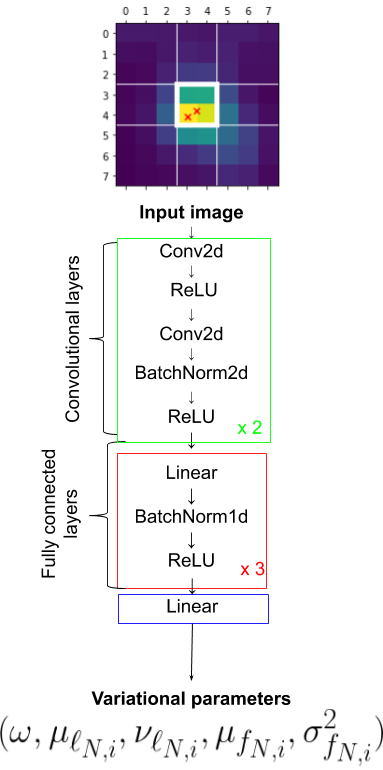
\includegraphics[width=0.4\textwidth]{figures/starnet_archetecture2.png}
    \vspace{-0.5cm}
    \caption{The neural network returning parameters for the variational distribution on each 2 x 2 image tile.}
    \label{fig:starnet_arch}
\end{figure}

Consider the output dimension of the neural network. The categorical parameter $\omega$ lies on the 
simplex and has dimension $N_{max} + 1$; for each $i = 1, ..., N$ and $N = 1, ..., N_{max}$, the location has a mean and variance on each coordinate; the flux has a mean and variance for each band. Thus, for star indexed by $(i, N)$, 
there are $2 \times (B + 2)$ parameters for its variational distribution. In total, the neural network has output dimension $(N_{max} + 1) + (B + 2) \times (N_{max}^2 + N_{max})$. 

Thus, decomposing the inference problem from full images into $2 \times 2$ tiles controls the output dimension of the neural network. 
On a crowded starfield with $H = W = 100$, $N$ is on the order of $10^3$, 
and $N_{max}$ must be larger. 
On the $2\times 2$ tile, we set $N_{max} = 3$. 
Moreover, the tiling amortizes the inference across image tiles: the same neural network is reused for each tile. 

We note however, that while the variational distribution factorizes over $2 \times 2$ tiles, we are not breaking the inference problem on the full image into embarrassingly parallel subproblems. We always evaluate the likelihood (when example, when computing the ELBO, equation~\eqref{eq:elbo}) on the full image. 
Light from a star within a 2 x 2 tile spills over into neighboring tiles, so the likelihood does not decouple into image tiles. 
